\documentclass{article}
\usepackage{graphicx} % Required for inserting images

\begin{document}

\begin{center}
{\Large MIDDLE EAST TECHNICAL UNIVERSITY\\
DEPARTMENT OF COMPUTER ENGINEERING\\}

\vspace{1cm}

{\huge \textbf{SUMMER PRACTICE REPORT\\
CENG400\\}}
\end{center}

\vspace{1cm}

{\large \noindent
\textbf{STUDENT NAME:} Batuhan Akçan\vspace{0.3cm}\\
\textbf{ORGANIZATION NAME:} METU ImageLab\vspace{0.3cm}\\
\textbf{ADDRESS:} Department of Computer Engineering, Middle East Technical University, Üniversiteler Mah. Dumlupinar Blv. No: 1 06800 Çankaya/Ankara\vspace{0.3cm}\\
\textbf{START DATE:} 01/07/2024\vspace{0.3cm}\\
\textbf{END DATE:} 23/08/2024\vspace{0.3cm}\\
\textbf{TOTAL WORKING DAYS:} 40\\}

\vspace{1cm}

\noindent
\textbf{STUDENT'S SIGNATURE}
\hspace{1.5cm}
\textbf{ORGANIZATION APPROVAL}

\newpage

\tableofcontents
\newpage

\section{INTRODUCTION}
\hspace{0.5cm}
This is the summer practice report for the internship that I have completed at METU ImageLab (Figure \ref{1}) in July and August of 2024.\\

The internship was conducted remotely, but there were meetings held in-person once a week. We (myself, and 5 other interns) have done our individual tasks during a week, and in a meeting, we presented what we did in the previous week and also were assigned our new tasks for the next week by Prof. Dr. Sinan Kalkan, our supervisor.\\

Each intern was assigned a different project to be worked on during the entire internship. My project was Transfer Learning for Heating Energy Prediction, of which details will be explained in later sections. Also, details about the organization and a summary of my internship experience will be shared.

\newpage

\section{INFORMATION ABOUT PROJECT}
\hspace{0.5cm}
The description of the project was as follows: Training a deep network to predict heating energy consumption of buildings requires a tedious data collection stage where precise 3D modeling and computationally expensive physical simulations are required. A practical solution for this challenge is to adapt a network pre-trained for heating energy estimation for a different city -- a.k.a., transfer learning. This task will explore novel strategies for performing transfer learning from a deep network trained for city A to city B.\\

In the upcoming pages, I will explain what I have done during the internship week by week.

\subsection{Week 1}
\hspace{0.5cm}
In the first week, I was not responsible for the given project. Instead, as a warm-up for the internship, a dataset containing heating energy consumption of some governmental buildings in Ankara in 2020 was provided by the supervisor in order for us to train. Our task was to train this dataset and get the highest R-squared (R2) score possible.\\

There were 32 features in the dataset. Numeric features included: form factor of the building, floor area of the building, width to depth ratio, unit with respect to north, south, west and east, sky exposure from north, south, west and east, number of people using the building, light density coming from sun to the building, total surface area of walls, windows, roof and floor, boiler efficiency, annual sum heating degree days, annual average dry bulb temperature, annual average of global horizontal irradiation. There was only a single categorical feature, which was infiltration. Labels of the dataset were heating end use and indoor overheating degree (IOD). The dataset included 63497 data samples.\\

During implementation phase, I have firstly loaded the necessary libraries, which were Tensorflow (Figure \ref{5}) (for training deep neural networks), Scikit-learn (Figure \ref{6}) (for machine learning), Pandas (Figure \ref{7}) (for data manipulation), Numpy (Figure \ref{8}) (for numerical computation), and Matplotlib (Figure \ref{9}) (for plotting results). Then, I have loaded the dataset with Pandas' $read\_csv()$ function. After that, I needed to do data preprocessing because there were some unnecessary features of which value is the same for all data, that were Annual Sum Heating Degree Days, Annual Average Dry Bulb Temperature, and Annual Average of Global Horizontal Irradiation. There were exactly the same for all data because the data is obtained from a single city, which is Ankara. So I dropped these features. Also, as a part of data preprocessing, I have separated numeric and categorical data, scaled the numeric data (in order for the model to work faster), one-hot encoded the categorical data (in order for model not to infer anything from decimal numbers), and then re-united the numeric and categorical data. Also, I have separated output labels from input features and scaled them as well.\\

After that, I have splitted the dataset into train and test sets, in order to see whether the model can generalize well on new data. I have placed 70\% of the data in train set, and the remaining 30\% in test set. Next, I continued with data visualization phase. Since the dataset size was too large, using t-SNE algorithm for dimensionality reduction would require too much time. That is why I have used Principal Component Analysis (PCA) algorithm to reduce the dimensionality of the data to 2 for visualizing purposes. The visualization of features are in Figure \ref{2} and labels are in Figure \ref{3}.\\

Then, I have put the data in a linear regression model. Training R2 score was 73.3\%, and test R2 score was 72.9\%. These results were not enough of course, that is why I tried neural network models afterwards.\\

As a neural network model, I firstly tried a 3 layered model. Each layer was a dense layer because I was not processing images or sequential data, but instead numerical data. Activation function was ReLU for hidden layers, linear for output layer. I tried layer size of 16, 4 and 2 units for the initial model. Compiled the model with mean squared error loss, Adam optimizer with learning rate 0.1, and trained it for 20 epochs. As a result, I obtained 74.5\% train R2 score and 74.3\% test R2 score. Results were not satisfactory.\\

To further increase R2 scores, I increased the number of layers. 5 layers with units 24, 16, 8, 4, 2 respectively. All configurations were the same, except that I trained it with learning rate 1e-2 for 20 epochs, and 1e-3 for another 20 epochs, and 1e-4 for another 20 epochs. So I applied a manual learning rate decay in a sense. 92.7\% train R2 score was obtained.\\

In order to find out whether R2 score can be increase even further, I tried another model with 7 layers with 24, 20, 16, 12, 8, 4, 2 units respectively. All other configurations were the same. I obtained 93.2\% train R2 score and 92.9\% test R2 score. So, apparently, R2 score would not increase too much even if we try higher number of layers. That is why I stopped there because 93.2\% R2 score was a promising result.\\

Lastly, I did an error analysis and the result is in Figure \ref{4}. One can see that the decline of MSE ends after 40th epoch.\\

Also, in the first week, other than training the model, some papers provided by the supervisor were read, understood, and a summary of them were presented during the meeting. The papers were as follows:
\begin{itemize}
    \item Yuan Gao, Yingjun Ruan, Chengkuan Fang, Shuai Yin (2020). Deep learning and transfer learning models of energy consumption forecasting for a building with poor information data, Energy and Buildings, 223.
    \item Chen, Y., Tong, Z., Zheng, Y., Samuelson, H., \& Norford, L. (2020). Transfer learning with deep neural networks for model predictive control of HVAC and natural ventilation in smart buildings. Journal of Cleaner Production, 254.
    \item Ding, Y., Zhang, Q., Yuan, T., \& Yang, K. (2018). Model input selection for building heating load prediction: A case study for an office building in Tianjin. Energy and Buildings, 159, 254–270.
    \item Fan, C., Sun, Y., Zhao, Y., Song, M., \& Wang, J. (2019). Deep learning-based feature engineering methods for improved building energy prediction. Applied Energy, 240, 35–45.
    \item Fan, C., Sun, Y., Xiao, F., Ma, J., Lee, D., Wang, J., \& Tseng, Y. C. (2020). Statistical investigations of transfer learning-based methodology for short-term building energy predictions. Applied Energy, 262.
    \item Fang, X., Gong, G., Li, G., Chun, L., Li, W., \& Peng, P. (2021). A hybrid deep transfer learning strategy for short term cross-building energy prediction. Energy, 215.
\end{itemize}

\subsection{Week 2}
\hspace{0.5cm}
In week 2, I have started working on the actual project. The supervisor provided me some files from the previous year's intern, Şevval. My task was in that week was to reproduce the given code files without changing them and see whether I can get similar results to Şevval.\\

In the files, what I have encountered was that along with .csv files that contain data for Ankara, Erzurum and Izmir; there were a Python (Figure \ref{10}) file for each task, which were: Ankara, Ank-Erz, Ank-Izm, Erz-10, Erz-30, Erz-50, Erz-100, Izm-10, Izm-30, Izm-50, Izm-100, TL-Ank-Erz-10, TL-Ank-Erz-30, TL-Ank-Erz-50, TL-Ank-Erz-100, TL-Ank-Izm-10, TL-Ank-Izm-30, TL-Ank-Izm-50, TL-Ank-Izm-100, TL-Ank+Erz-Izm-10, TL-Ank+Erz-Izm-30, TL-Ank+Erz-Izm-50, TL-Ank+Erz-Izm-100, TL-Ank+Izm-Erz-10, TL-Ank+Izm-Erz-30, TL-Ank+Izm-Erz-50, TL-Ank+Izm-Erz-100. Let me explain each task in detail.
\begin{itemize}
    \item Ankara: Training of Ankara dataset.
    \item Ank-Erz: Training of Ankara and Erzurum datasets.
    \item Ank-Izm: Training of Ankara and Izmir datasets.
    \item Erz-10: Training of 10\% of Erzurum dataset.
    \item Erz-30: Training of 30\% of Erzurum dataset.
    \item Erz-50: Training of 50\% of Erzurum dataset.
    \item Erz-100: Training of 100\% of Erzurum dataset.
    \item Izm-10: Training of 10\% of Izmir dataset.
    \item Izm-30: Training of 30\% of Izmir dataset.
    \item Izm-50: Training of 50\% of Izmir dataset.
    \item Izm-100: Training of 100\% of Izmir dataset.
    \item TL-Ank-Erz-10: Transfer learning, which is applied as transferring knowledge gained from Ankara dataset into 10\% of Erzurum dataset.
    \item TL-Ank-Erz-30: Transfer learning, which is applied as transferring knowledge gained from Ankara dataset into 30\% of Erzurum dataset.
    \item TL-Ank-Erz-50: Transfer learning, which is applied as transferring knowledge gained from Ankara dataset into 50\% of Erzurum dataset.
    \item TL-Ank-Erz-100: Transfer learning, which is applied as transferring knowledge gained from Ankara dataset into 100\% of Erzurum dataset.
    \item TL-Ank-Izm-10: Transfer learning, which is applied as transferring knowledge gained from Ankara dataset into 10\% of Izmir dataset.
    \item TL-Ank-Izm-30: Transfer learning, which is applied as transferring knowledge gained from Ankara dataset into 30\% of Izmir dataset.
    \item TL-Ank-Izm-50: Transfer learning, which is applied as transferring knowledge gained from Ankara dataset into 50\% of Izmir dataset.
    \item TL-Ank-Izm-100: Transfer learning, which is applied as transferring knowledge gained from Ankara dataset into 100\% of Izmir dataset.
    \item TL-Ank+Erz-Izm-10: Transfer learning, which is applied as transferring knowledge gained from Ankara and Erzurum datasets into 10\% of Izmir dataset.
    \item TL-Ank+Erz-Izm-30: Transfer learning, which is applied as transferring knowledge gained from Ankara and Erzurum datasets into 30\% of Izmir dataset.
    \item TL-Ank+Erz-Izm-50: Transfer learning, which is applied as transferring knowledge gained from Ankara and Erzurum datasets into 50\% of Izmir dataset.
    \item TL-Ank+Erz-Izm-100: Transfer learning, which is applied as transferring knowledge gained from Ankara and Erzurum datasets into 100\% of Izmir dataset.
    \item TL-Ank+Izm-Erz-10: Transfer learning, which is applied as transferring knowledge gained from Ankara and Izmir datasets into 10\% of Erzurum dataset.
    \item TL-Ank+Izm-Erz-30: Transfer learning, which is applied as transferring knowledge gained from Ankara and Izmir datasets into 30\% of Erzurum dataset.
    \item TL-Ank+Izm-Erz-50: Transfer learning, which is applied as transferring knowledge gained from Ankara and Izmir datasets into 50\% of Erzurum dataset.
    \item TL-Ank+Izm-Erz-100: Transfer learning, which is applied as transferring knowledge gained from Ankara and Izmir datasets into 100\% of Erzurum dataset.
\end{itemize}

10-fold cross-validation method was applied for 400 experiments for each task by Şevval. Since my computer's GPU was limited in terms of performance, I have applied 10-fold cross-validation for only 10 experiments for each task, that is, I have trained the entire dataset only once. After that, I have saved the resultant .pt files. Also, I have written average train and test R2 scores of 10 experiments into an Excel file. The resultant R2 scores were a little lower than those of Şevval's, because of the fact that she did 400 experiments.

\subsection{Week 3}
\hspace{0.5cm}
In the third week, I was told to apply a fine-tuning method called Layer-Selective Rank Reduction (LASER) to reproduced models. The paper of the method can be accessed via: https://arxiv.org/abs/2312.13558.\\

Firstly, I have read and understood the paper. I have learned how it works, which layers we should apply it to, what should be the value of $k$ (a hyperparameter), etc. After that, from reproduced models, from those which were used for transfer learning, I chose those with the highest test R2 score ones and applied LASER to all layers of all of those models. Since $k$ is a hyperparameter, I needed to try different values of it and take the one that gives the highest accuracy. I have tried $k=0.1, 0.5, 0.9$ and found out that $k=0.9$ gives the best result. I have transferred results into an Excel file, as always.\\

Also, I have prepared a presentation that explains how LASER method works and presented it in the next meeting.

\subsection{Week 4}
\hspace{0.5cm}
In week 4, I was told that Şevval had applied LASER last year already, and my supervisor wanted me to get result files of those and compare them with my results. In the files, I saw that Şevval had tried $k$ values $0, 0.1, ..., 0.9, 1.0$. However, she applied LASER to basis models (Izm-X, Erz-X) and not to transfer learning models. Since I have applied LASER only to transfer learning models, there was nothing to compare. Another thing that I noticed was she applied LASER to each layer of all models individually, not all layers at once, despite the fact that it is suggested to apply it to all layers in the paper, which is what I did. Because of this, the resultant R2 scores I got was higher than her results.

\subsection{Week 5}
\hspace{0.5cm}
In the fifth week, I was requested to apply another fine-tuning method called Low Rank Adaptation (LoRA) to reproduced models. The paper of the method can be accessed via: https://arxiv.org/pdf/2106.09685.\\

As always, I firstly have read the paper and understood it. I have figured out what should be the rank $r$, which matrices should we apply it to, etc. As in applying LASER, from reproduced models, from those which were used for transfer learning, I chose those with the highest test R2 score ones and applied LoRA to all matrices of all of those models, which was recommended in the paper. I have tested $r=2,4,8,16,32$ hyperparameter values and found out that $r=32$ gives the best result. I have transferred results into an Excel file and presented a presentation that includes what LoRA is, how it works, advantages of using it, and results of its application to some well-known models, such as RoBERTa, DeBERTa, GPT-2, and GPT-3.

\subsection{Week 6}
\hspace{0.5cm}
In week 6, Prof. Sinan Kalkan wanted me to apply LoRA+ this time, which is yet another fine-tuning method. It is the acronym of Efficient Low Rank Adaptation and can be accessed via: https://arxiv.org/abs/2402.12354.\\

I have applied LoRA+ to all matrices of models that I have applied LoRA to.\\

In LoRA+, there is another hyperparameter called "Learning rate ratio". This is what we are trying to tune. In the paper, a wide range of values from 2 up until 800 were tried on some state-of-the-art models. As can be seen in the paper, values between 4 and 80 give better results. That is why, I tried $lr\_ratio=2,4,8,16,32$ on our reproduced models, where I used a fixed rank value $r=32$ since it gave the best result. Because, otherwise, the complexity of the problem would be $O(n^2)$, which would require too much time.\\

I obtained the best results with hyperparameter values $r=32, lr\_ratio=4, ß_1=0.9, ß_2=0.999, \epsilon=1e-6$ where I optimized with AdamW, an optimization algorithm.\\

As always, results were extracted into an Excel file and a presentation that explains LoRA+ was presented.

\subsection{Week 7}
\hspace{0.5cm}
In the seventh week, professor wanted me to read LoRA and LoRA+ papers in more detail and understand them altogether. I have read them more carefully, understood, and presented their mathematical background, how they work in the background, what are advantages and disadvantages of using them, state-of-the-art models that they were applied to by other people, results of applying them, etc.

\subsection{Week 8}
\hspace{0.5cm}
In the last week, professor wanted me to apply 400 experiments with all fine-tuning methods, instead of 10 experiments in order to more effectively compare my results to Şevval's results. Since this would require much more time, I have applied 400 experiments only to TL-Ank+Erz-Izm-X models. I have tried only the hyperparameter values that gave the best result, i.e, $k=0.9$ for LASER, $r=32$ for LoRA, and $lr\_ratio=4$ for LoRA+. Among the three methods, I have obtained the best result with LoRA+.
\newpage

\section{ORGANIZATION}
\hspace{0.5cm}
ImageLab is a research lab at the Department of Computer Engineering, Middle East Technical University. Research in this lab focuses on image and video analysis, computer vision, machine learning, deep learning and image processing. The lab was founded by Prof. Neşe Yalabık and Prof. Fatoş Yarman Vural in 1994. Since then, the members of the lab have produced numerous master’s and doctoral theses, and scientific publications.\\

The lab currently hosts several funded research projects that are led by five principal investigators, who are: Assoc. Prof. Emre Akbaş, Prof. Fatoş Yarman Vural, Assoc. Prof. Gökberk Cinbiş, Assoc. Prof. Hande Alemdar, and Prof. Sinan Kalkan. Among them, Prof. Sinan Kalkan was my supervisor throughout the internship.\\

Website of the organization can be accessed via this link:\\ https://image.ceng.metu.edu.tr/index.html
\newpage

\section{CONCLUSION}
\hspace{0.5cm}
In conclusion, the internship was a great experience. It made me gain experience working as an AI Engineer. I have learned some fine-tuning methods and some Python libraries (Tensorflow, PyTorch, Scikit-learn etc.) which are widely used in the industry. It also made me recall my former knowledge about statistics, calculus, and linear algebra. With this internship, I have broadened my knowledge in machine learning and deep learning areas (for instance, I have learned how k-fold cross validation works). Also, this internship has shown me how academia is. I know that things that I have done in the internship are closely related to being a researcher in an academic institution, so if I decide to enroll in a MSc in Computer Engineering in the future, this internship will be a great reference for me.
\newpage

\section{APPENDIX}
\begin{figure}[h]
    \centering
    \includegraphics[width=1\linewidth]{YMYgaRmn_400x400.jpg}
    \caption{METU ImageLab}
    \label{1}
\end{figure}
\begin{figure}
    \centering
    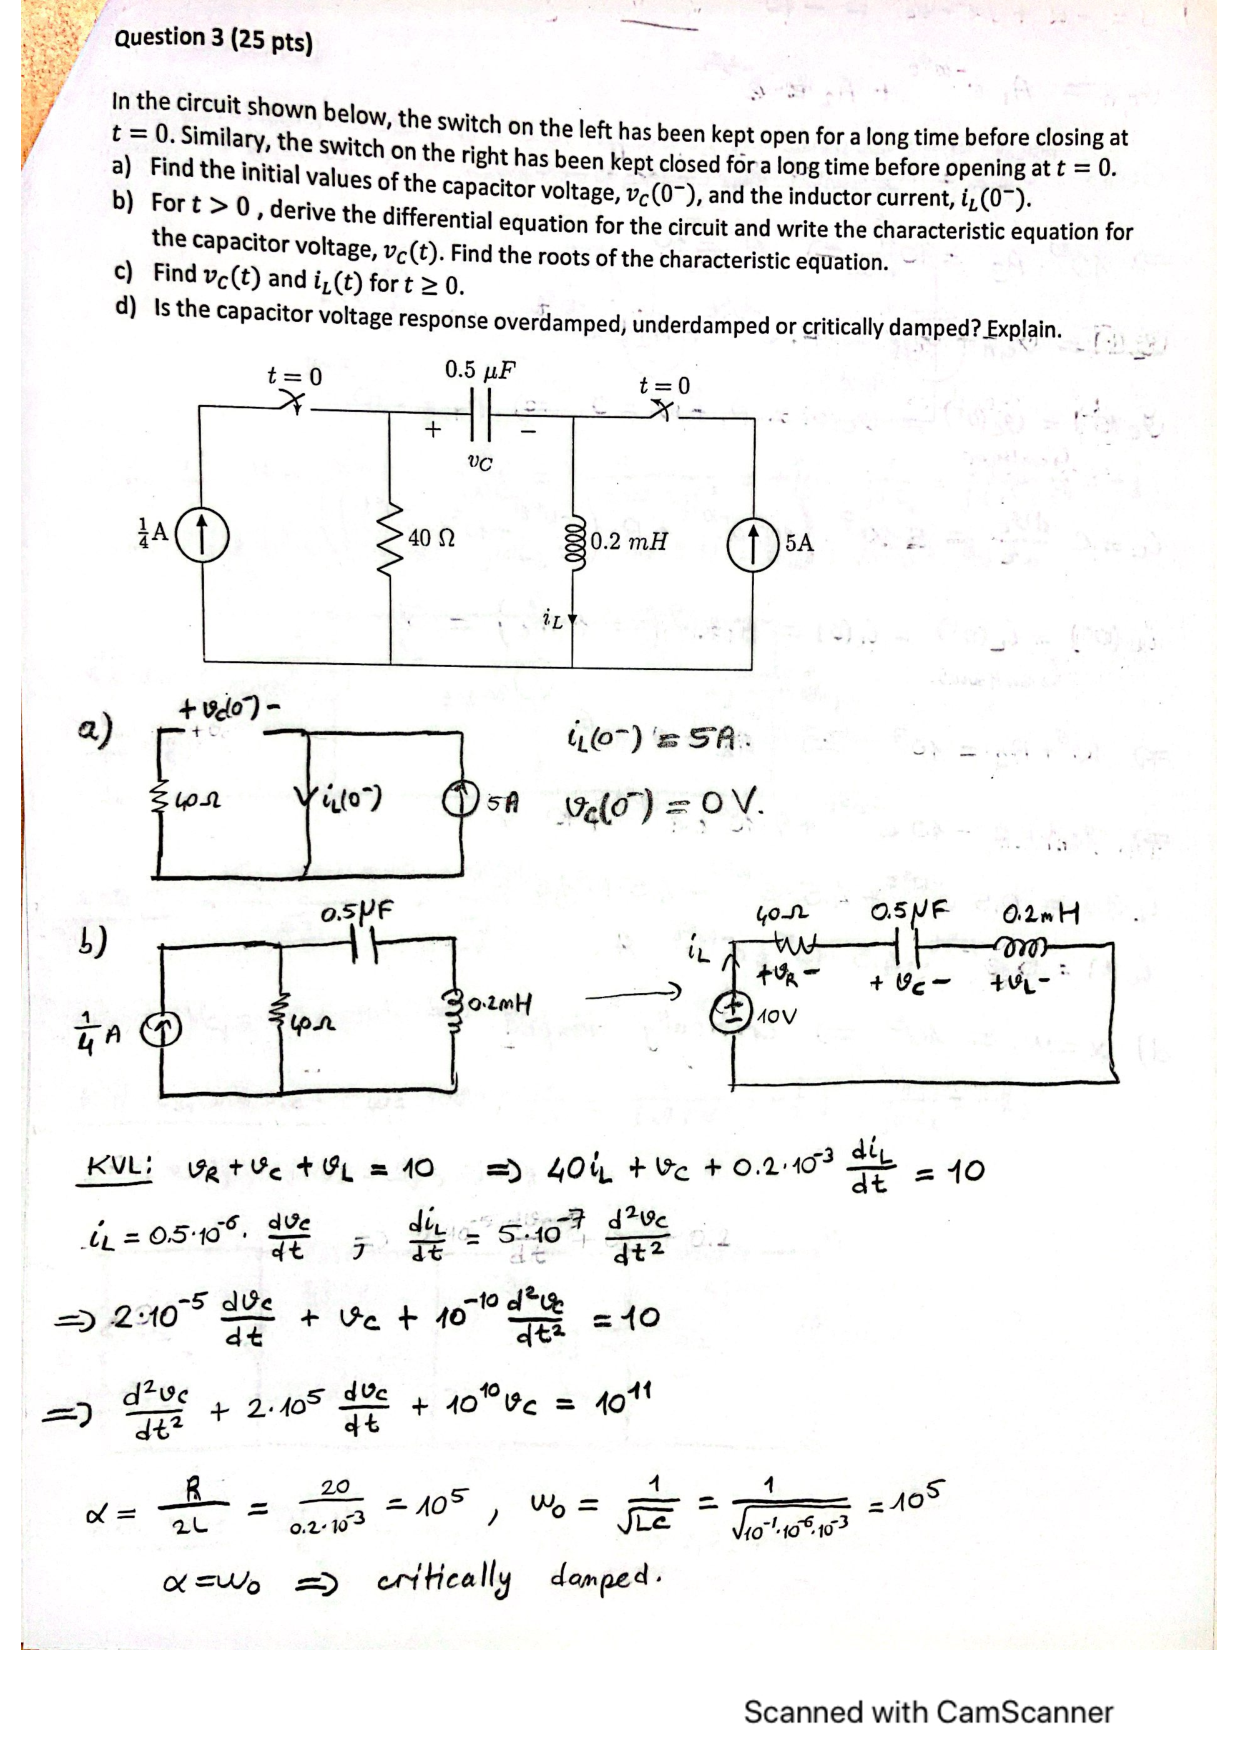
\includegraphics[width=1\linewidth]{5.png}
    \caption{Tensorflow, a Python library for training deep neural networks}
    \label{5}
\end{figure}
\begin{figure}
    \centering
    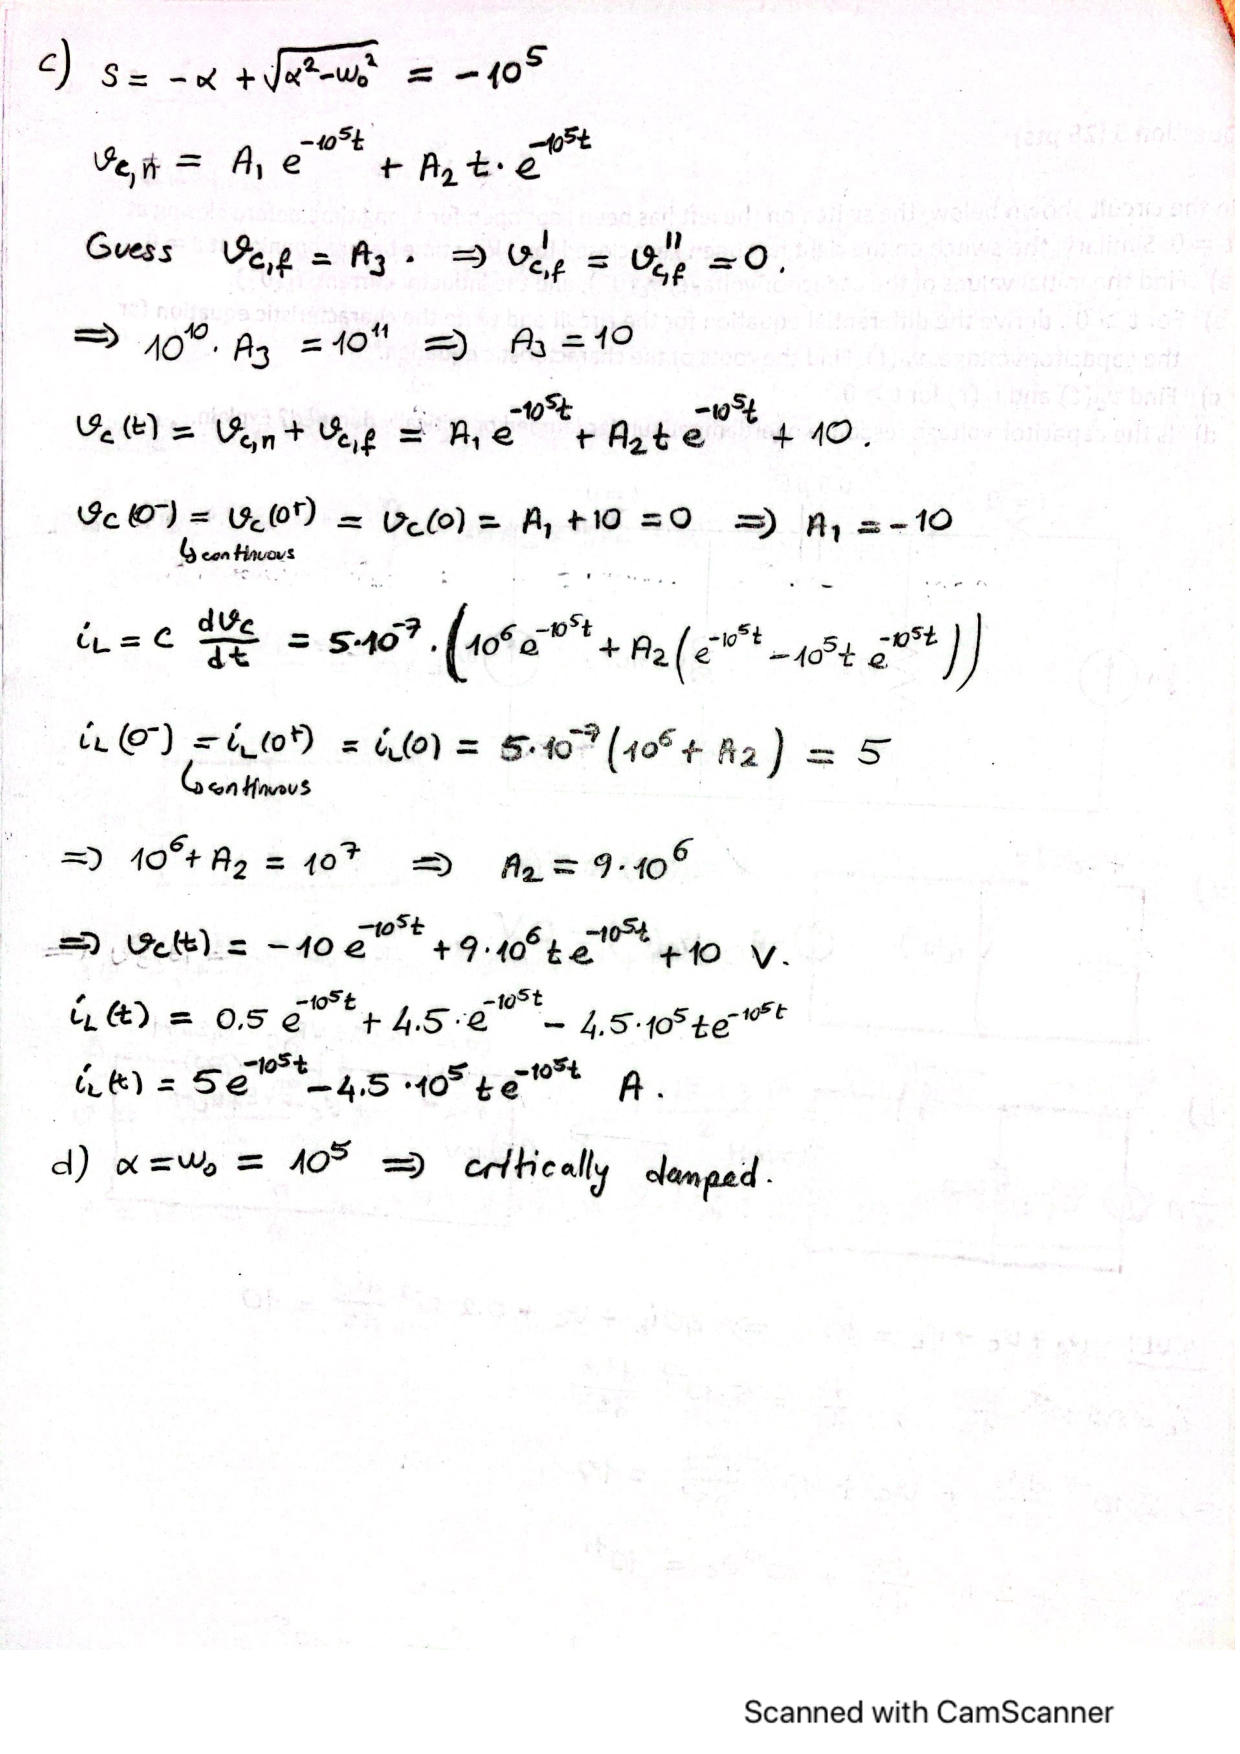
\includegraphics[width=1\linewidth]{6.png}
    \caption{Scikit-learn, a Python library for machine learning}
    \label{6}
\end{figure}
\begin{figure}
    \centering
    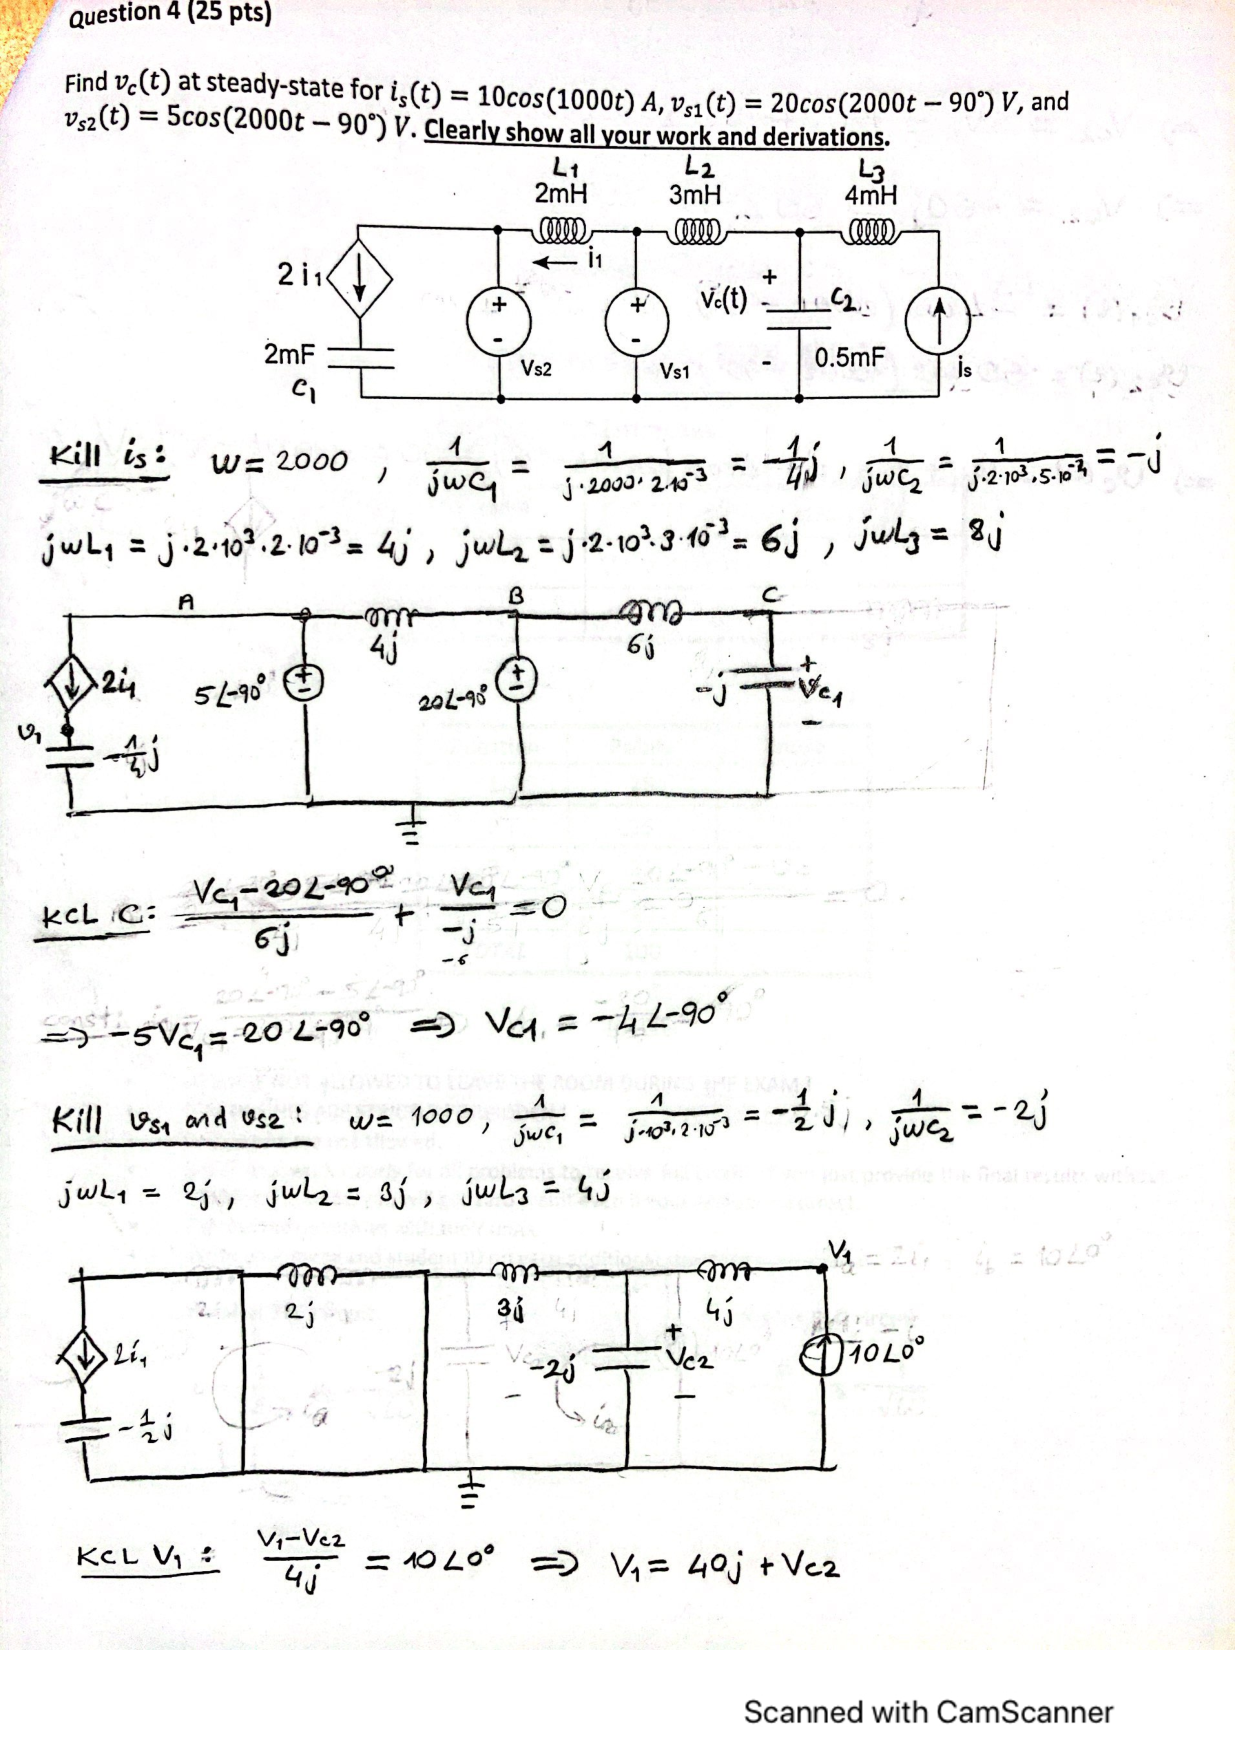
\includegraphics[width=1\linewidth]{7.png}
    \caption{Pandas, a Python library for data manipulation}
    \label{7}
\end{figure}
\begin{figure}
    \centering
    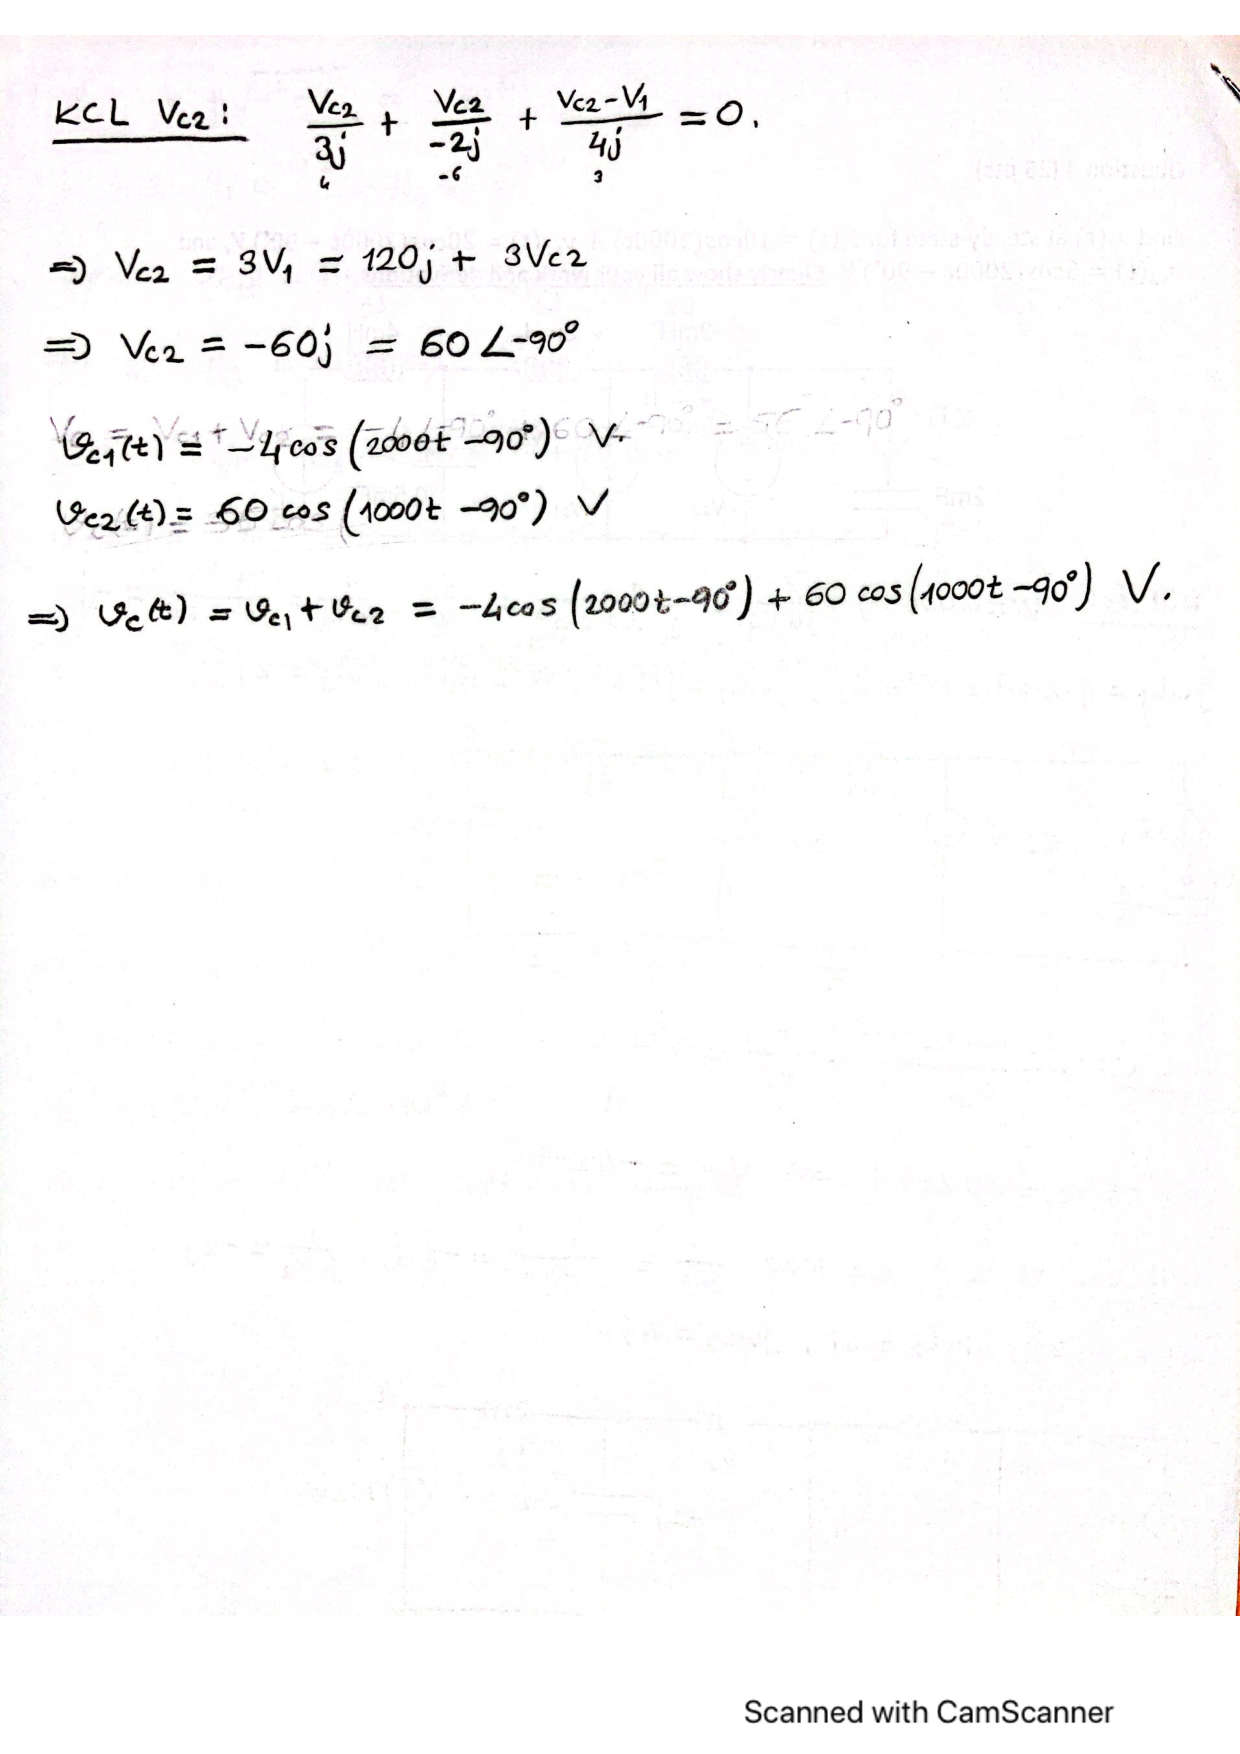
\includegraphics[width=1\linewidth]{8.png}
    \caption{Numpy, a Python library for numerical computation}
    \label{8}
\end{figure}
\begin{figure}
    \centering
    \includegraphics[width=1\linewidth]{9.png}
    \caption{Matplotlib, a Python library for data visualization}
    \label{9}
\end{figure}
\begin{figure}
    \centering
    \includegraphics[width=1\linewidth]{asd.png}
    \caption{Visualization of train and test set features}
    \label{2}
\end{figure}
\begin{figure}
    \centering
    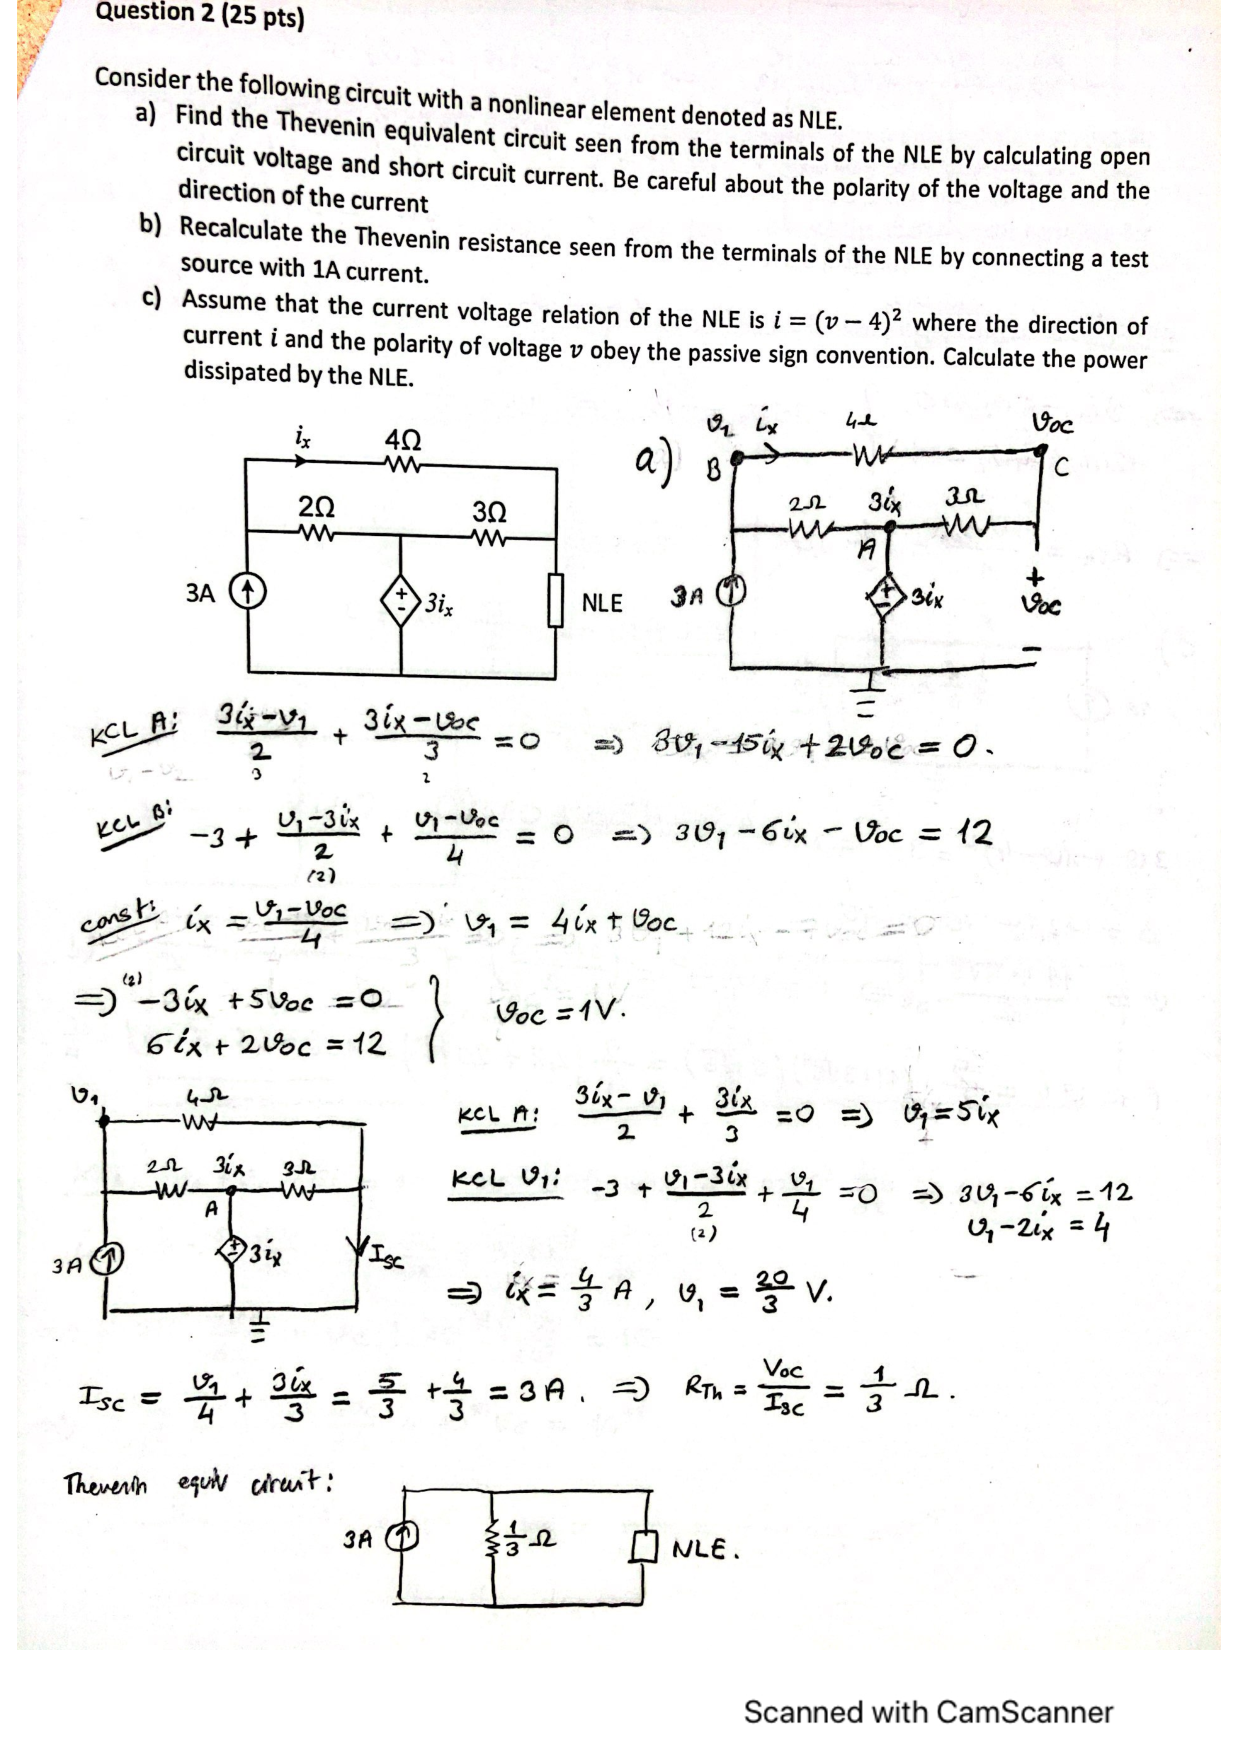
\includegraphics[width=1\linewidth]{3.png}
    \caption{Visualization of train and test set labels}
    \label{3}
\end{figure}
\begin{figure}
    \centering
    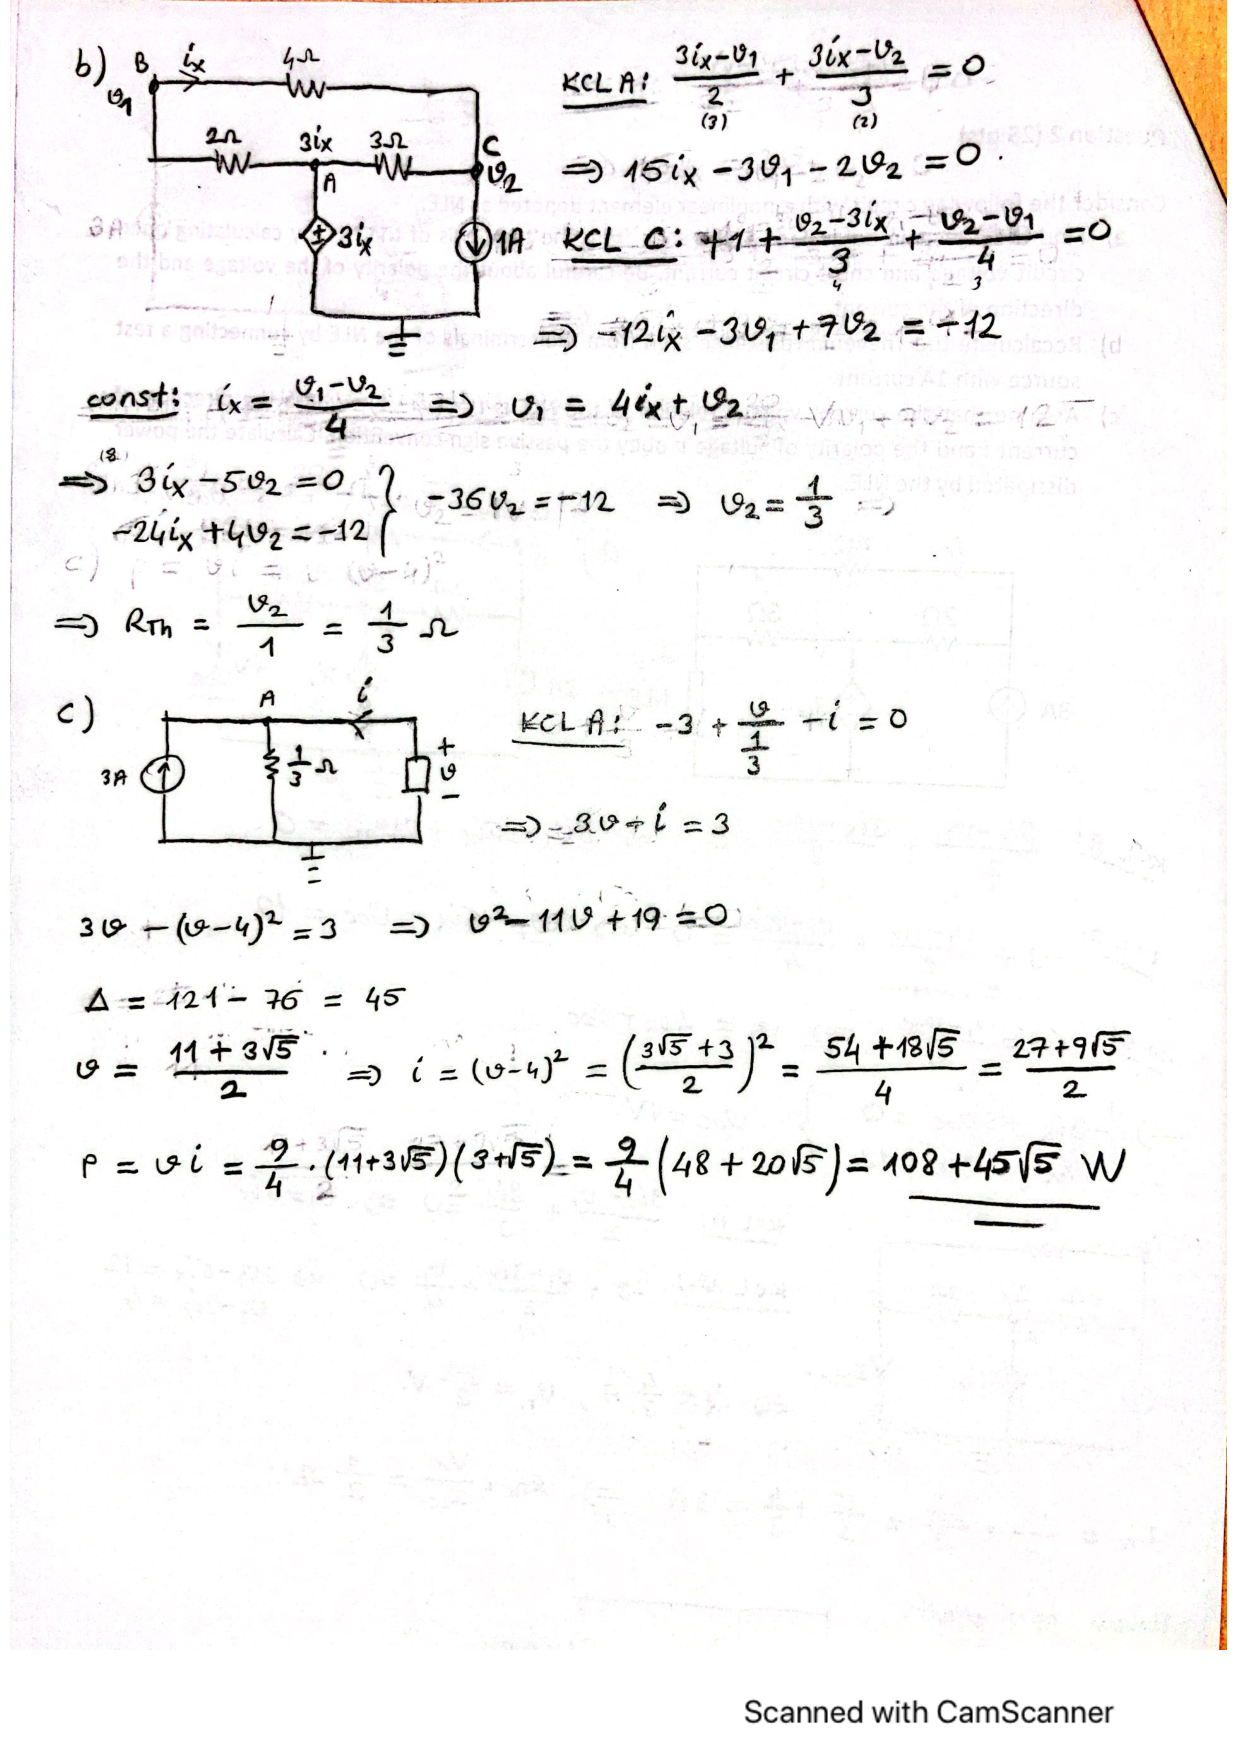
\includegraphics[width=1\linewidth]{4.png}
    \caption{Error Analysis}
    \label{4}
\end{figure}
\begin{figure}
    \centering
    \includegraphics[width=1\linewidth]{10.png}
    \caption{Python, a high-level, dynamically-typed, general-purpose programming language}
    \label{10}
\end{figure}

\end{document}